\chapter{Defining A Scene}

In this chapter we first see how to lay out different objects into a
virtual world, something that we call a scene.
We also see how we use our scene data during our rendering operations.
Finally, we set up and render a simple scene to demonstrate the
concepts discussed in this chapter.

\begin{figure}[ht]
    \centering
    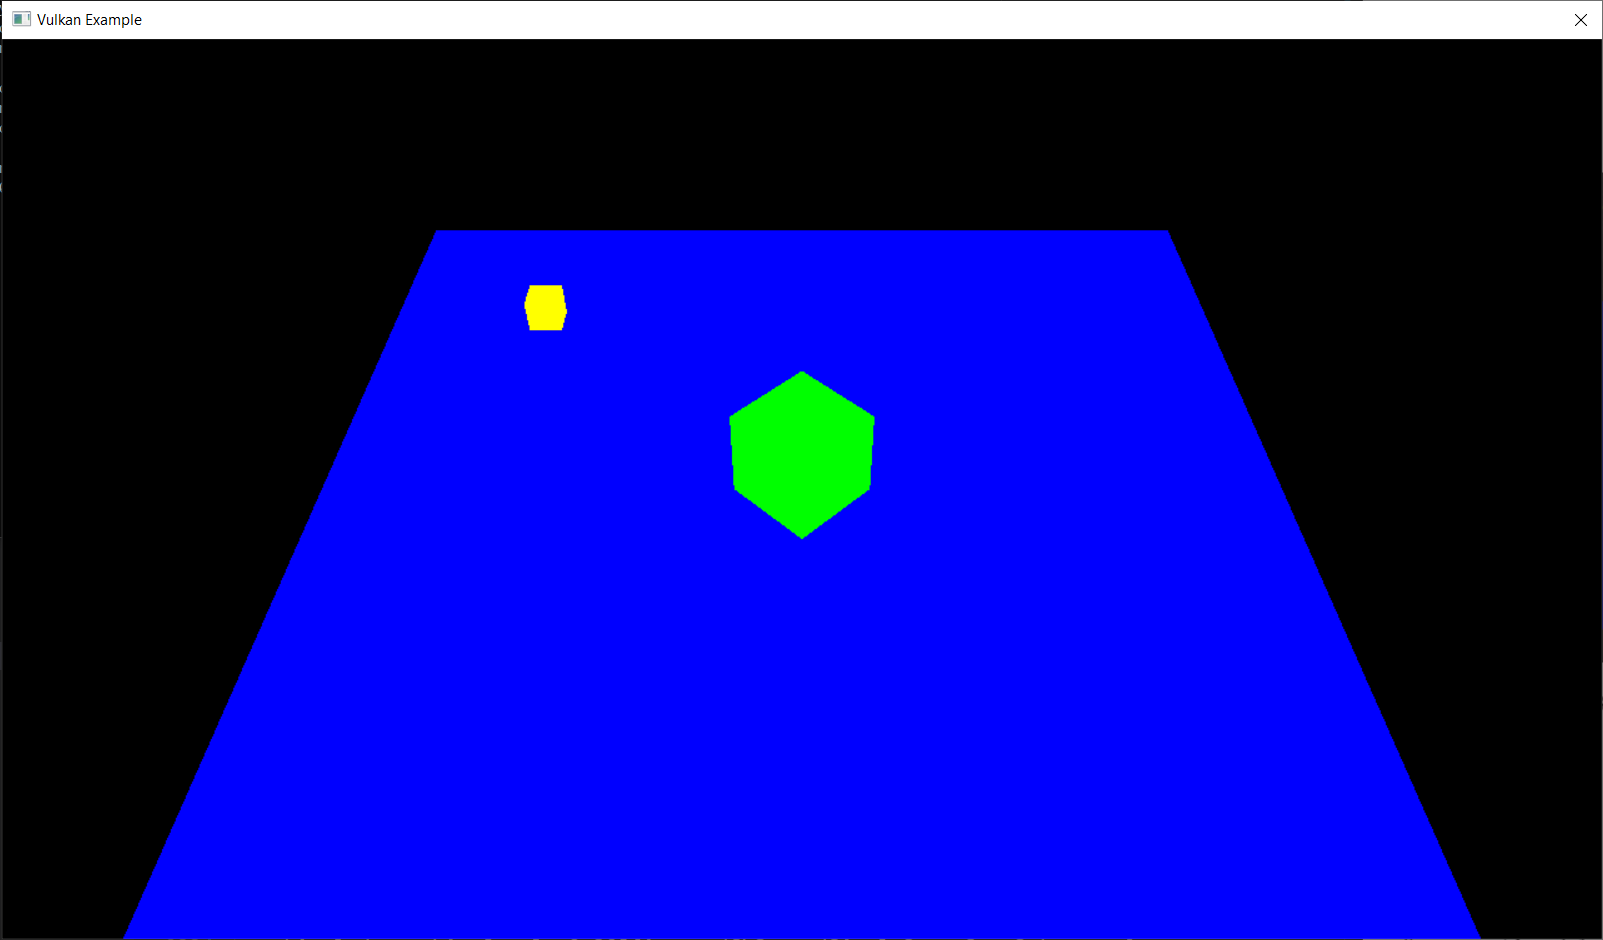
\includegraphics[scale=0.20]{images/ChScene/SimpleScene.png}
    \caption{Define and render a simple scene}
    \label{fig::SimpleScene}
\end{figure}

\section{Entities}

We define a scene as a collection of entities.
An entity is a bundle of all the data that is necessary to place
an object inside a scene and to render it.

\subsection{Placing Entities Inside A Scene}

Entities can be placed all around a scene.
We can have a cube placed at $(0, 0, 0)$, the origin of our scene.
Another cube located at $(5, 3, 0)$ could be rotated by $30$
degrees around the $x$ axis and by $60$ degrees around the $z$ axis.
Another cube could be scaled by a factor of $10$ around all its three axis,
thus making it bigger than our other cubes.
From this description, we can see that our entities have three main properties:
\begin{itemize}
    \item a 3d vector that represents its position inside the scene
    \item a 3d vector that represents its rotations around the $x, y$ and $z$ axis
    \item a scalar that represents its scale
\end{itemize}



\section{Rendering Entities}
